\documentclass[10pt,twocolumn,legalpaper,draft]{article}

%//////////////////////////////////////////////////////////////////////////////////////
\textwidth 17cm             	%Define el ancho del texto, por página.
\textheight 29cm            	%Define el alto del texto, por página.
\topmargin -1,5cm           	%Define el margen superior del texto, por página.
\leftmargin 0cm             	%Define el margen izquierdo del texto, por página.
\pagestyle{empty}           	%Define el tipo de numeración usada. Nula en este caso.
\parindent 1,5em            	%Define el tamaño de la identación usada en el documento.
\usepackage[final]{graphicx}       	%Se incluye el paquete para insertar las imágenes.
\usepackage[utf8]{inputenc}	%Se incluye el paquete para usar acentos
%///////////////////////////////////////////////////////////////////////////////////////


\begin{document}



%TITULO
%//////////////////////////////////////////////////////////////////////////////////////
\title{\textbf{\huge{Robot Seguidor de Línea con Sistema de Control basado en Red Neuronal}}}
\author{Emanuel Sánchez \\
\normalsize{Estudiante de la Universidad Simón Bolívar -- Venezuela}}
\date{}                       %date coloca la fecha del documento. De no ponerse,se
\pagestyle{empty}                               %coloca por defecto la fecha de última compilación.
\maketitle                    %Crea el título usando las opciones de \title \author y
\thispagestyle{empty} 
                              %\date                             
%///////////////////////////////////////////////////////////////////////////////////////

%EL ABSTRACT
\textbf{\textit{Abstract--- } Hoy en día la robótica desempeña un papel fundamental en el desarrollo tecnológico. Esta área del conocimiento ha brindado al ser humano la capacidad de materializar su deseo de construir artefactos que simplifiquen y automaticen la realización de diversas tareas. En este mismo orden de ideas, las competencias nacionales de robótica que se han desarrollado en el país durante los últimos 5 años han tenido como objetivo promover la innovación mediante la integración de diferentes áreas de conocimiento. \newline \newline \indent Por esto,} \emph{Mach Five} \textbf{surge como una propuesta de alto nivel que cumpla con los requerimientos necesarios para participar en la} \emph{VI Competencia Nacional de Robótica USBBots 2016.}\newline
% \textbf{dentro de la categoría} \emph{Velocista}. \newline
\vspace{0,8em}
%EL ABSTRACT

%LA INTRODUCCION
\centerline{\Large{\textbf{\sc{I. introducción}}}} 
\vspace{0,8em}
Este año la categoría \emph{Velocista} de la competencia nacional posee nuevos desafíos, el objetivo de la misma es diseñar y construir un robot autónomo que recorra cierta pista en el menor tiempo posible, sin embargo, la dificultad radica en que en esta oportunidad la pista tiene bifurcaciones las cuales serán señalas mediante marcas que indican la dirección a tomar. No tomar correctamente una bifurcación puede conllevar a un loop infinito, a un camino más largo o un extremo muerto. Además, la pista cuenta con tramos en los que la línea a seguir puede estar ausente una cierta distancia. \newline
\vspace{0,8em}
%LA INTRODUCCION

%EL ROBOT
\centerline{\Large{\textbf{\sc{II. el robot}}}}
\vspace{0,8em}

Con base en los requerimientos de la competencia se realizó el diseño de \emph{Mach Five} teniendo como objetivo los siguientes puntos:

\begin{itemize}
	\item[$\rightarrow$]\textbf{Detección Óptima:} de la línea, bifurcaciones y marcas a través de una matriz de sensores IR.
	\item[$\rightarrow$]\textbf{Procesamiento de alto desempeño:} sistemas de adquisición y procesamiento óptimos que permitan mayor velocidad del robot.
	\item[$\rightarrow$]\textbf{Motores de alta velocidad:} capaces de funcionar con un alto rendimiento de acuerdo a la capacidad de procesamiento.
	\item[$\rightarrow$]\textbf{Diseño liviano:} chasis y tarjetas integradas optimizadas para permitir mayor velocidad del robot.
\end{itemize}

\begin{center}
	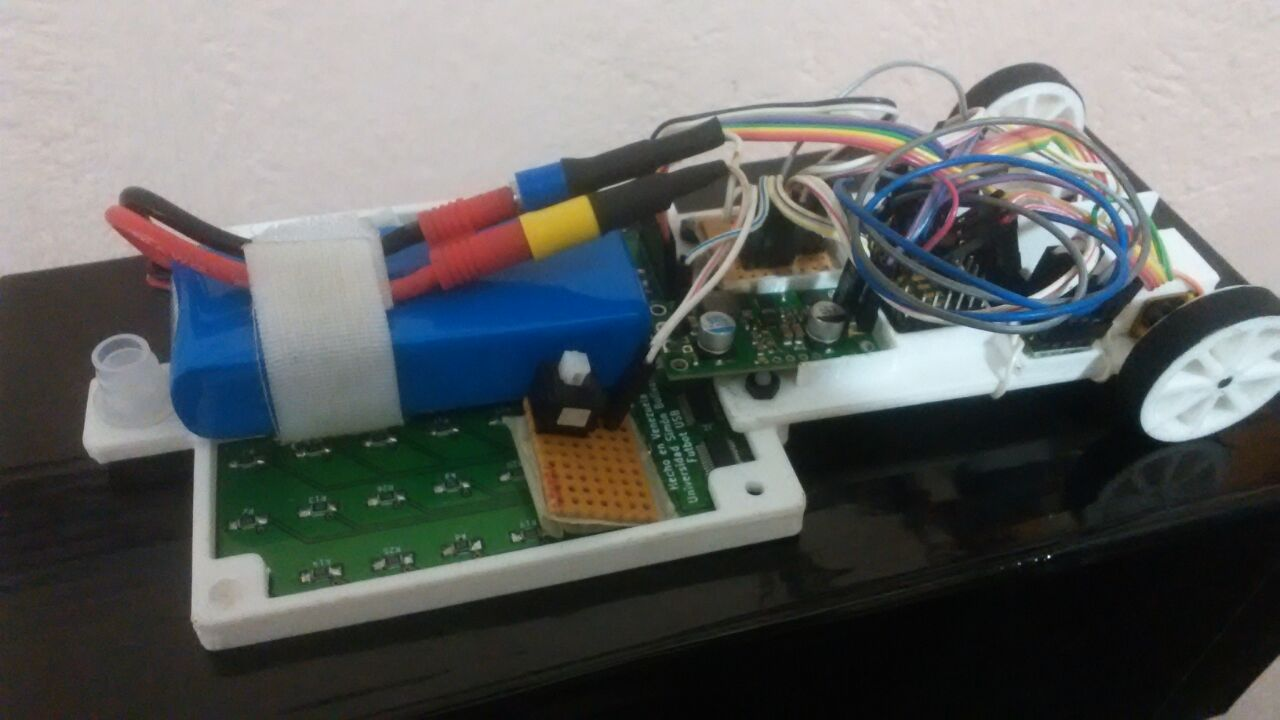
\includegraphics[scale=0.18]{Robot}
	
	\textit{Figura 1: Prototipo Mach-Five semi armado}
\end{center}

A continuación se presenta una descripción más profunda del robot: \newline

%%HARDWARE
\centerline{\Large{\textbf{\sc{1. Hardware}}}}
\vspace{0,8em}

El prototipo consiste en una plataforma (chasis) impreso en 3D con PLA (Poliácido Láctico), sobre el cuál estarán dispuestos los siguientes módulos que componen el robot:\newline

\textit{\textbf{1.a.- Teensy 3.2:}}
es una tarjeta de desarrollo que cuenta con un procesador ARM Cortex M4 de 32 bits. Este es el centro de procesamiento de todo el robot, en este microcontrolador se toman todas las decisiones de alto y bajo nivel. En el se realiza primero la adquisición y acondicionamiento de los datos de todos los sensores, para que luego el sistema de control pueda realizar las operaciones necesarias. \newline \indent
La elección de este micro se debe a su gran capacidad de procesamiento, además, ofrece muchas ventajas al momento de su programación ya que cuenta con una gran diversidad de librerías muy optimizadas.\newline

\textit{\textbf{1.b.- Micro Motores High Power Pololu 6V:}}
es un pequeño motor de alta potencia con escobillas de carbón de larga duración capaz de lograr 3000 RPM a 120 mA sin carga. Cuenta con una extensión de eje para añadir un encoder. Además, posee ofrece un torque suficiente para mover el peso total del robot con un excelente desempeño.\newline

\textit{\textbf{1.c.- Encoders Opticos Pololu:}}
Estos van soldados en la parte trasera de cada motor. Provee una cantidad de 20 ticks por revolución y son de suma importancia para el sistema de control ya que proporcionan datos para obtener la velocidad del motor.\newline

\textit{\textbf{1.d.- Controlador de motores Pololu DRV8838:}}
Es un controlador "puente H" miniatura que puede manejar una corriente de hasta 1.7A. Ofrece excelentes opciones para controlar un motor DC mediante una configuración de velocidad y dirección. Además, posee protección contra voltaje-reverso, sobre-corriente y exceso de temperatura.\newline

\textit{\textbf{1.e.- Matriz de Sensores detectores de línea:}}
Es, como su nombre lo indica, una matriz de 7x7-1 sensores de línea analógicos, sin embargo la tarjeta cuenta con convertidores ADC que entregan los datos resultantes mediante comunicación SPI. A pesar de los 48 sensores que incluye ofrece una rápida adquisición de los datos correspondiente a cada uno de ellos. Cabe destacar que este dispositivo fue desarrollado por los integrantes de la agrupación FutBot de la Universidad Simón Bolívar.\newline

\begin{center}
		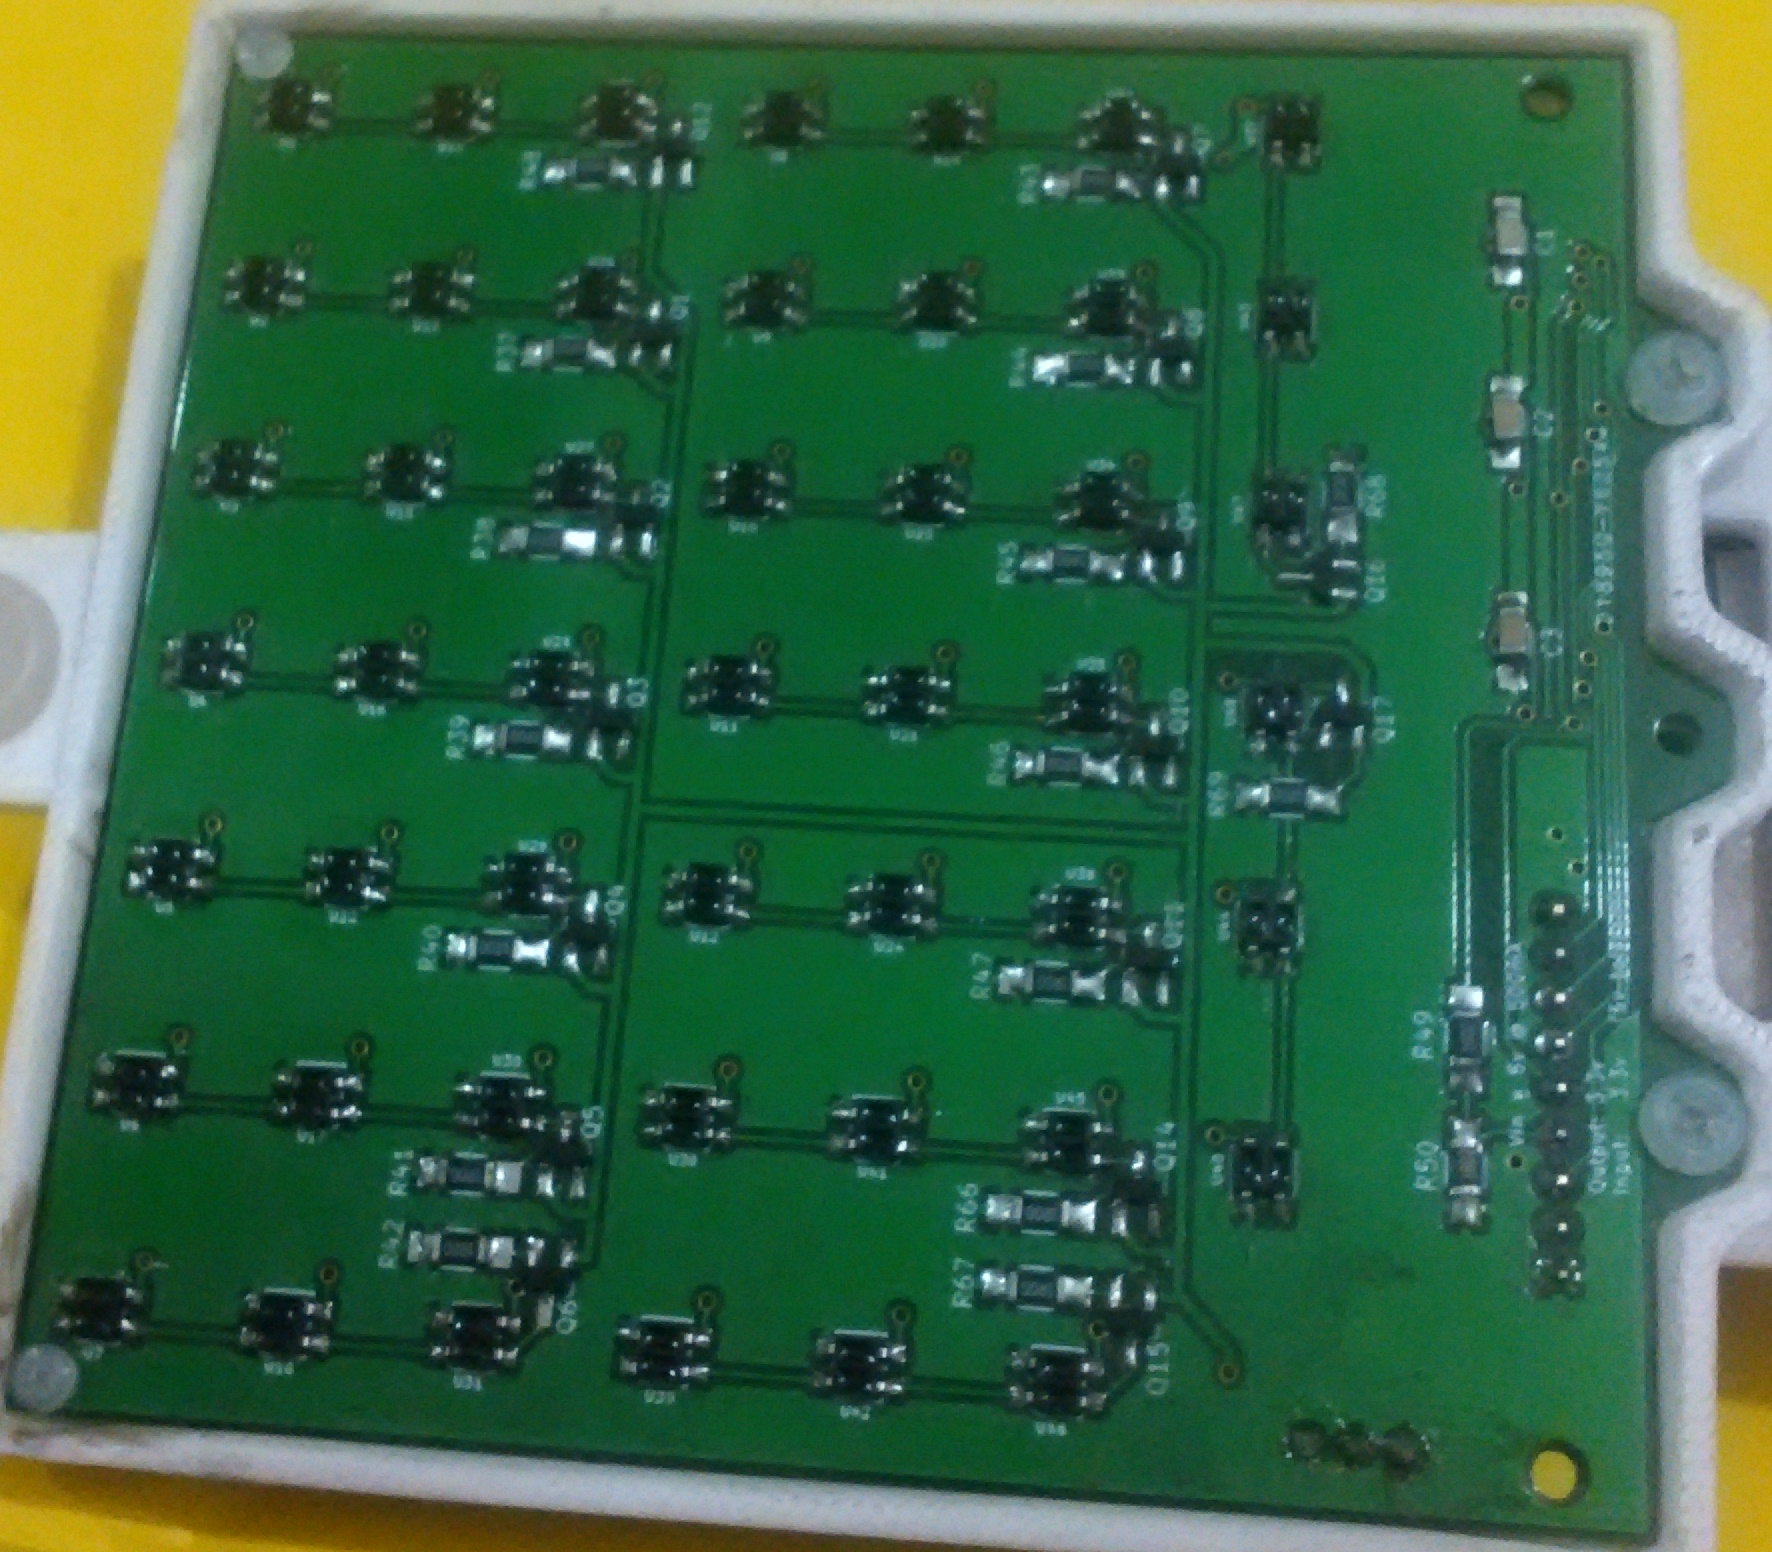
\includegraphics[scale=0.09]{matriz1}
		
		\textit{Figura 2: Matriz de Sensores}
\end{center}

\textit{\textbf{1.f.- Pantalla LCD:}}
Se decide incluir esta para generar un sistema de debugeo y calibración de la matriz de sensores.\newline

\textit{\textbf{1.g.- Fuente de alimentación:}}
Debido a que todo el sistema trabaja a +3.3V y 5V se hace uso de una batería LiPo de 7.4V con 2100mAh, la cual ofrece una buena relación peso-potencia y garantiza el máximo rendimiento del robot durante la competencia con una sola carga.\newline \indent

Además de la batería se usa para alimentar todos los módulos (sensores, microcontrolador, etc) un regulador switching step-down de 5V y 6A el cual ofrece buen manejo de potencia con una alta eficiencia (80\% - 95\%). Además, evita el recalentamiento excesivo.\newline
\vspace{0.8em}

\begin{center}
	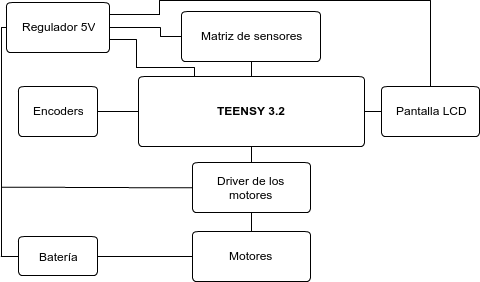
\includegraphics[scale=0.49]{Hardware}
	
	\textit{Figura 3: Hardware del Sistema}
\end{center}


%%HARDWARE

%%SOFTWARE
\centerline{\Large{\textbf{\sc{2. Software}}}}
\vspace{0,8em}

\textit{\textbf{2.a.- Sitema de control principal:}}
El sistema de control propuesto esta basado en una \emph{Red Neuronal} la cuál trabajará como clasificador de casos para cada uno de los cuales hay acciones específicas.\newline
En primer lugar se realiza la adquisición de la matriz de sensores la cual genera en cierta forma una "imagen" de 7x7 pixeles en escala de grises. Esta información es pasada a través de una red neuronal la cual clasifica las entradas en los siguientes casos:

\begin{itemize}
	\item[$\rightarrow$] Línea Continua (recta o curva).
	\item[$\rightarrow$] Línea Segmentada.
	\item[$\rightarrow$] Bifurcación.
	\item[$\rightarrow$] Pre-Bifurcación.
\end{itemize}

\begin{center}
	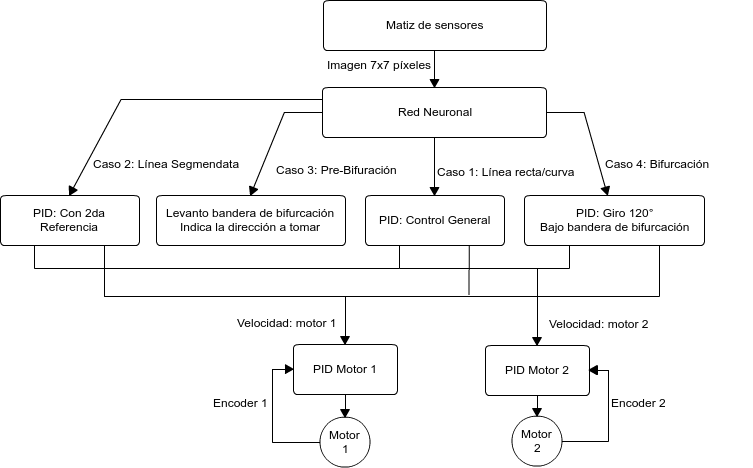
\includegraphics[scale=0.31]{Software}
	
	\textit{Figura 4: Sistema de Control}
\end{center}

Para cada uno de estos casos hay un respuesta predeterminada, por ejemplo, para la línea recta y curva el sistema de control usa tres PID, uno para mantener la alineación del robot con la recta/curva en base a la primera fila de sensores, y los otros dos para garantizar la velocidad correcta en cada motor.\newline

Por otro lado, el caso de "Pre-bifurcación" se da cuando el robot está sobre una marca que indica la dirección a tomar en la próxima bifurcación, de este modo el sistema levanta una bandera indicando una pronta bifurcación y otra señalando la dirección a tomar. Así, cuando sucede el caso "Bifurcación" es porque el robot está justo sobre la misma y entonces el sistema genera las señales necesarias para dar un giro de 120$^{\circ}$ en la dirección correspondiente.\newline

Por último, en el caso de "Línea Segmentada" el sistema levanta una bandera de modo que el PID que mantiene la alineación de con la recta/curva no considera sólo la primera fila de sensores sino también la última. De este modo, el sistema no pierde la referencia.\newline
\vspace{0,8em}
%%SOFTWARE

%EL ROBOT

%PROBLEMAS ENCONTRADOS
\centerline{\Large{\textbf{\sc{III. Problemas Encontrados}}}}
\vspace{0,8em}
A continuación se presenta una descripción de las principales dificultades enfrentadas durante el diseño y creación del robot Mach Five, además de la propuesta o solución correspondiente:

\begin{itemize}
	\item[$\rightarrow$]\textbf{Chasis:} Elaboración de un chasis liviano para cumplir con el límite de peso que puede mover los motores con un excelente desempeño.\newline
En primer lugar se pensó en un chasis hecho de aluminio, pero posteriormente de decidió que la impresión en 3D con PLA era más liviana, mantenía la rigidez necesaria y además simplificaba el proceso de construcción.
	\item[$\rightarrow$]\textbf{Alimentación:} se presentaron dificultades con el regulador de voltaje debido a que todo el sistema tenía un consumo de aproximadamente 1.5A, lo que producía un recalentamiento excesivo en el regulador usado antes de la propuesta final (el mencionado en la descripción del hardware). Primero se intentó solucionar haciendo uso de disipadores, sin embargo, al no obtener resultados aceptables se decidió hacer uso del regulador descrito anteriormente en el inciso de descripción de Hardware.\newline
\end{itemize}

\vspace{0,8em}
%PROBLEMAS ENCONTRADOS

%RECOMENDACIONES
\centerline{\Large{\textbf{\sc{IV. Recomendaciones}}}}
\vspace{0,8em}

Se recomienda en primer lugar dedicar el tiempo suficiente a la profunda investigación en cada una de las áreas (electrónica, mecánica y computación) que se necesitan para el desarrollo del prototipo. Además de una correcta planificación del trabajo a realizar.\newline

También se recomienda iniciar el trabajo de diseño y construcción en un periodo no menor a tres meses para poder garantizar un lapso tiempo adecuado dedicado a la realización de pruebas para poder así generar correcciones y optimizaciones importantes.\newline
\vspace{0,8em}
%RECOMENDACIONES

%CONCLUSIONES
\centerline{\Large{\textbf{\sc{V. Conclusiones}}}}
\vspace{0,8em}

El diseñó del robot \emph{Mach Five} para que cumpliera con las especificaciones de la competencia implicó un reto debido a que el equipo de la agrupación FutBot deseaba desarrollar una plataforma de alto nivel, capaz de ser extrapolada a competencias internacionales.\newline

Durante las largas y exhaustivas horas de trabajo se hizo notorio la necesidad de dedicar tiempo e investigación profunda en el desarrollo y planificación. Por otro lado se pudieron comprobar muchos conocimientos simplemente teóricos.\newline

Definitivamente los objetivos de la competencia nacional de robótica de este año se cumplen al generar un ambiente de innovación y desarrollo de nuevas soluciones mediante la implantación de retos distintos a los presentados en años anteriores.\newline

La integración de diversas áreas de conocimiento como la electrónica, mecánica y computación propician el desarrollo de nuevos conocimientos y el trabajo en equipo.\newline

\vspace{0,8em}
%CONCLUSIONES

\end{document}

